\documentclass{article}
\usepackage[utf8]{inputenc}
\usepackage{amsmath}
\usepackage{graphicx}
\graphicspath{ {./images/} }

\newcommand{\figref}[1]{Figure \ref{#1}}

\title{Minimum Perimeter-Sum Bipartition Implementation}
\author{Allen Mi, Haakon Flatval}
\date{December 2018}

\begin{document}

\maketitle

\begin{abstract}
    The Minimum Perimeter-Sum Bipartition problem is stated as follows: Given set of points in the Euclidean plane, partition it into two subsets such that the sum of perimeters of their convex hulls is as small as possible. In this text, we describe our implementation of the algorithm by Abrahamsen et al \cite{abrahamsen_mpsb} and provide analyses on its behaviour given different inputs.
    % Fill in more here / rewrite abstract as things happen
\end{abstract}

\section{Introduction}
The Minimum Perimeter-Sum Bipartition problem is the problem of dividing a set of point in the two-dimensional plane into two subsets $P_1$ and $P_2$ such that the sum of the perimeters of $\text{CH}(P_1)$ and $\text{CH}(P_2)$ is minimized, where $\text{CH}(P)$ is the convex hull of the set of points $P$. In 2017, Abrahamsen et al  \cite{abrahamsen_mpsb} devised an algorithm that solves this problem in time $O(n \log^4 n)$. 

% Fill out more details about bounds and related work - like in the algorithmic paper?

We provide an implementation of this algorithm \cite{implementation} and an overview on how the implementation is structured. Furthermore, we give an analysis of how different input sets affect the performance of the algorithm, and discuss our method of constructing such input sets.
% This might have to be rewritten at some point

\section{Background}

% Description of the problem and the algorithm

\section{Implementation}

\subsection{Hierarchy of Subroutines}

% Dependency information of the subroutines
\begin{figure}[ht]
    \centering
    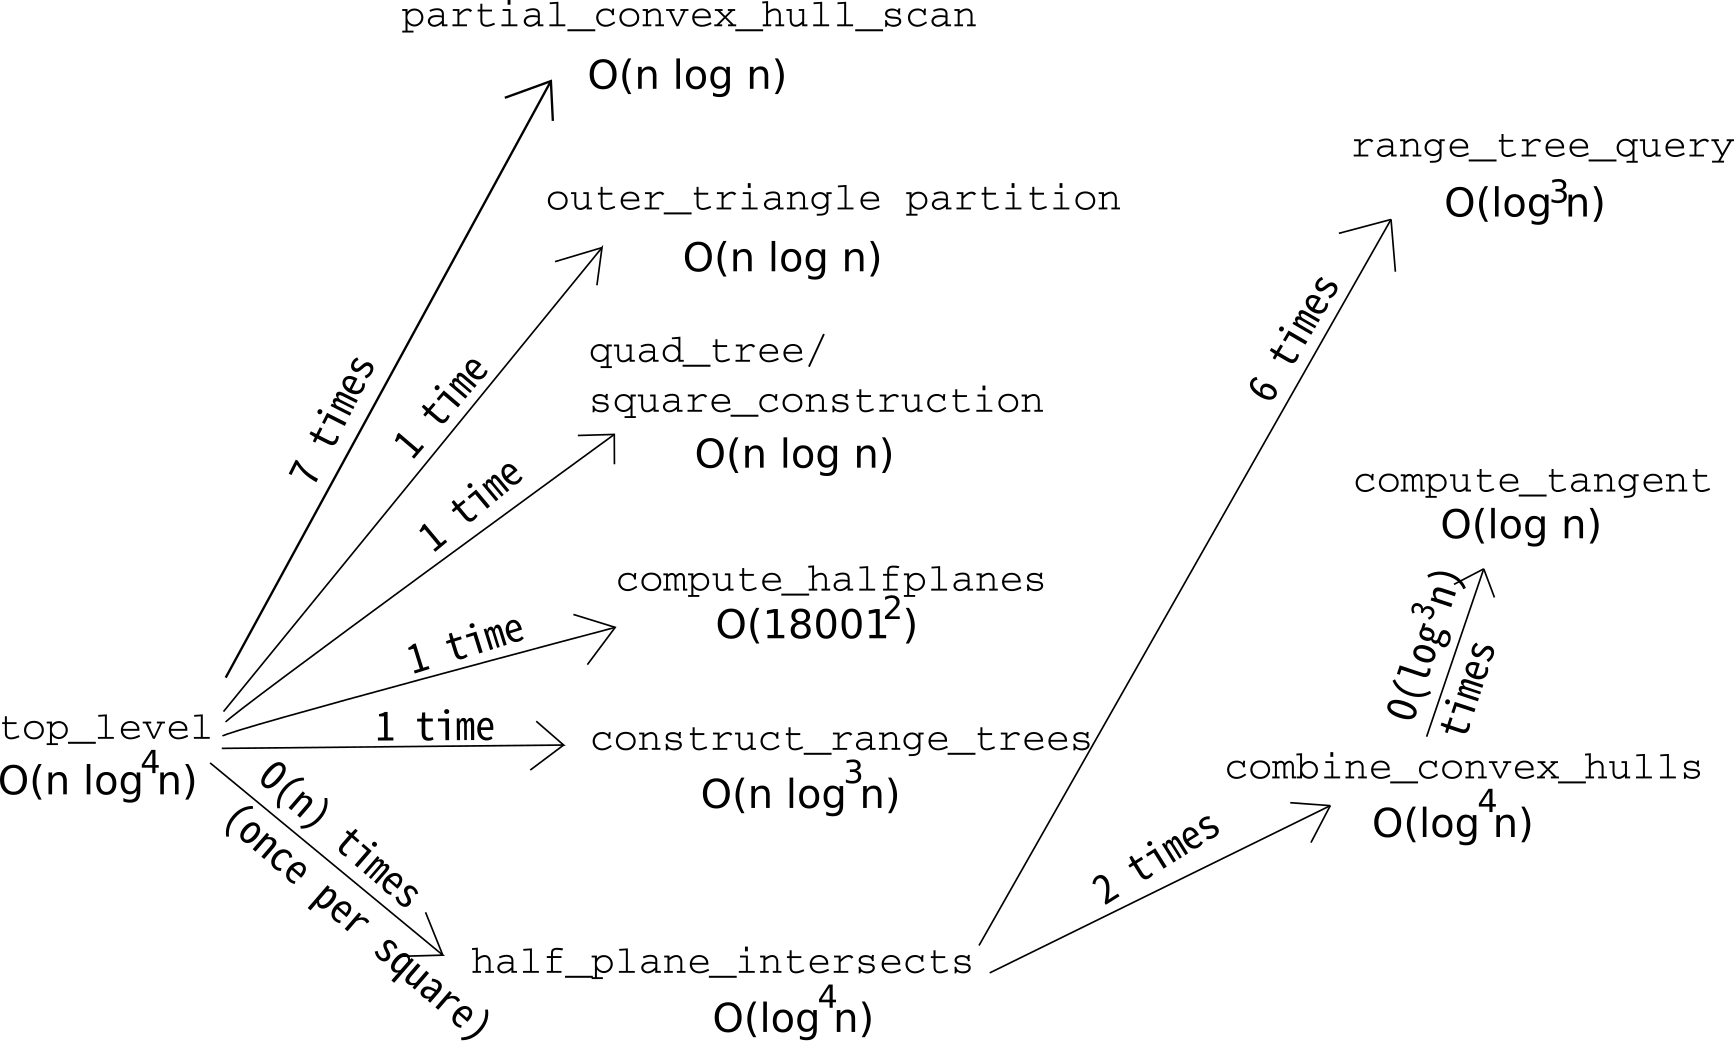
\includegraphics[width=\textwidth]{hierarchy}
    \caption{Structural hierarchy of subroutines}
    \label{fig:hierarchy}
\end{figure}

The structural hierarchy of the subroutines for this algorithm is outlined in \figref{fig:hierarchy}.

\subsubsection{Partial Convex Hull Scan}

\textit{For a given angle $\phi$ and a set of points $P$, this subroutine computes the upper and lower halves of the convex hull of $P$, scanning through the nodes like in Graham's scan, but along a line with angle $\phi$ to the x-axis. This allows us to quickly compute convex hulls of a bipartition of $P$ separated by a line perpendicular to the scan direction. This operation takes $O(n \log n)$ time for a given angle, $n$ being the size of $P$.}

\subsubsection{Outer Triangle Partition}

\textit{For a given set of points $P$, computes all triangles formed by three successive points on the set's convex hull, and finds and stores the subset of the points contained in each such triangle. This allows us to quickly compute the length of the convex hull of $P \ {p}$, where $p$ is a point on the convex hull of $P$. This operation takes $O(n \log n)$ time, where $n = |P|$.}
    
\subsubsection{Quad Tree Construction} 
\textit{Each node in such a quad tree represents a square in the plane. Each node has four children, representing the regions of the four equal squares that make up their parent's region. The construction of a compressed quad tree over $n$ points takes $O(n \log n)$ time. (Given appropriate computational model)}

\subsubsection{Range Tree Construction and Search}
\textit{The range tree we construct here has three levels. The first level sorts the points on the x-axis, the subsequent level sorts the points at each node by the y-axis. The lowest level sort the points by a given direction in the plane. This allows us to easily find points that are restricted to a given rectangular axis-aligned region in the plane, and that are also inside a specified half-plane. This range tree also compute the convex hull of each node in the lowest level of the range tree. The range tree construction takes $O(n\log^3n)$, $n$ being the number of points over which we construct the tree}

\subsubsection{Tangent Computation}
\textit{For two polygons $A$ and $B$, computes their tangents using the algorithm provided in \cite{kirkpatrick}. We use this to determine which polygons belongs to the hull in the \textit{Convex Hull Combining} subroutine. The algorithm uses $O(\log(a + b))$ time, where $a$ and $b$ are the number of points on the boundary of $A$ and $B$ respectively.}

\subsubsection{Convex Hull Combining}
\textit{For a given set of convex hulls $\mathcal{C}$, finds the convex hull of all points on all the hulls. We use this to combine the convex hulls found from a query in the range tree described above, including its length, so that we can evaluate the perimeter. The running time for this subroutine is $O(k \log m)$, $k$ being the number of convex polygons, and $m$ the number of points on the hulls in total.}

\section{Performance}

% Performance analysis of each subroutine, as well as the entire algorithm. The sample input of the performance analysis could be from uniform sampling of the target rectangular region.

\section{Input Design}

\subsection{Input in Realistic Scenarios}

% Use random sampling with 2-d normal distribution. We can calculate the standard deviation on either axis by limiting the expected position on either side of an axis to be equal to that of the uniform distribution.

\subsection{Adversarial Inputs}

% Leverage the O(n log(n)) / O(n log^4(n)) distinction

\subsection{Input Generation via Gradient Descent}

% Experimental input generation

\section{Conclusion}

\begin{thebibliography}{}
\bibitem{abrahamsen_mpsb}
Mikkel Abrahamsen, Mark de Berg, Kevin Buchin, Mehran Mehr, and Ali D. Mehrabi. Minimum Perimeter-Sum Partitions in the Plane, \textit{33rd International Symposium on Computational Geometry} (SoCG 2017)

\bibitem{kirkpatrick}
D. Kirkpatrick and J. Snoeyink. Computing common tangents without a separating line. \textit{Proc. 2nd Workshop Alg. Data Struct. (WADS),} LNCS 955, pages 183-193, 1995

\bibitem{implementation}
Allen Mi, Håkon Flatval. \textit{Minimum Perimeter-Sum Bipartition implementation} \texttt{https://github.com/AllenGlan/mpsb-implementation}


\end{thebibliography}
\end{document}
